% SynthMRI paper draft. Build: cd paper && latexmk -pdf main.tex  (or: pdflatex, bibtex, pdflatex x2)
% Every number is copied from docs/RESULTS.md / docs/results_tables.md (regenerated by scripts/collect_results.py).
\documentclass[10pt,a4paper]{article}
\usepackage[margin=22mm]{geometry}
\usepackage[T1]{fontenc}
\usepackage[utf8]{inputenc}
\usepackage{lmodern}
\usepackage{microtype}
\usepackage{graphicx}
\usepackage{booktabs}
\usepackage{array}
\usepackage{multirow}
\usepackage{placeins}
\usepackage{amsmath,amssymb}
\usepackage[numbers,sort&compress]{natbib}
\usepackage[font=small,labelfont=bf]{caption}
\usepackage{xcolor}
\usepackage[colorlinks=true,linkcolor=blue!60!black,citecolor=blue!60!black,urlcolor=blue!60!black]{hyperref}
\graphicspath{{../docs/figures/}}

\newcommand{\todo}[1]{\textcolor{red}{[#1]}}
\newcommand{\ldm}[1]{\textsc{ldm-#1}}
\newcommand{\dice}[1]{#1}

\title{Latent Diffusion for Synthetic Brain MRI:\\An Exploratory Evaluation of Fidelity, Memorisation, and Segmentation Utility}
\author{Wasiq Nauman Qureshi\and Syed Muhammad Hamza Shah\thanks{University of Miami}}
\date{}

\begin{document}
\maketitle

\begin{abstract}
Synthetic brain MRI could expand scarce labelled datasets, but realistic-looking images alone do not show that a generation pipeline is viable. An exploratory assessment must also ask whether samples resemble held-out data without copying training images, retain diversity, respond to unseen tumour masks, and show at least conditional downstream utility. We do not propose a new architecture. Instead, we evaluate a conventional mask-conditioned 2-D latent diffusion model (LDM) on BraTS~2020 using patient-level splits, validation-based early stopping, a nearest-neighbour memorisation check, held-out fidelity and diversity metrics, unseen-patient masks, and segmentation as a secondary stress test. The evidence is mixed. Without regularisation, FID continues to improve while the model memorises: by epoch~200, 97\,\% of samples lie closer to a training slice than real held-out slices do. Cached affine augmentation postpones this failure and yields the best early-stopped model (validation FID 24.7 vs 29.9). At 256\,px, the selected model reaches FID 10.45 against a 9.55 floor between two real sets and generates from unseen tumour masks with little loss in fidelity, providing encouraging distributional evidence within this dataset. Practical utility is conditional. Mixing synthetic slices into segmenter training lowers mean Dice by $0.030$--$0.036$ at 128\,px, whereas synthetic pre-training gains $+0.021$ / $+0.014$ over a compute-matched control at 10\,\% / 25\,\% real data, and 256\,px mixing gains $+0.027$ with 26 real patients. Autoencoder controls are consistent with the latent bottleneck being the principal limitation at 128\,px. Within this 2-D BraTS setting, latent diffusion is therefore a plausible research pipeline, but its viability depends on resolution, regularisation, checkpoint selection and how the samples are used; clinical realism and broad utility are not established.
\end{abstract}

\section{Introduction}
Synthetic images are an attractive response to the scarcity of labelled medical data, and denoising diffusion models~\citep{ho2020ddpm,rombach2022ldm} have produced increasingly realistic brain MRI samples~\citep{pinaya2022brain,khader2023ddpm3d,kazerouni2023survey}. The practical question, however, is not simply whether a sample looks convincing. For this exploratory study, \emph{viability} means that an established generation pipeline can be trained reproducibly, produces samples that resemble held-out data while remaining diverse and distinct from the training set, responds to unseen tumour masks, and shows enough conditional utility to justify further investigation. These criteria are deliberately narrower than anatomical validity, diagnostic usefulness or clinical readiness, none of which is evaluated here.

We do not introduce a new generator architecture or optimisation method. Instead, we use a conventional mask-conditioned LDM to map the evidence for and limits of synthetic brain MRI generation on BraTS~2020. The objective is exploratory, while the evaluation rules are pre-declared to reduce cherry-picking: patient-level splits, validation-based checkpoint selection, a flip-aware nearest-neighbour memorisation check, model selection without test data, and three seeds with patient-matched pairs for the secondary segmentation assessment. The study asks four questions:
\begin{itemize}\setlength\itemsep{1pt}
  \item How do training length, regularisation and checkpoint selection affect fidelity and memorisation (Sect.~\ref{sec:mem})?
  \item Do selected models produce diverse samples that resemble held-out data and respond to tumour masks from unseen patients (Sect.~\ref{sec:gen})?
  \item How do image resolution and the pretrained autoencoder constrain the evidence for viability (Sect.~\ref{sec:256}, \ref{sec:decoder})?
  \item As a secondary test, when do synthetic image--mask pairs help or hurt downstream segmentation (Sect.~\ref{sec:seg}--\ref{sec:secondary})?
\end{itemize}
The paper's contribution is therefore an empirical assessment of feasibility and boundary conditions rather than a claim of architectural novelty.

\section{Related work}
\paragraph{Diffusion models for medical image synthesis.} \citet{pinaya2022brain} trained a 3-D LDM on 31,740 UK Biobank brains; \citet{khader2023ddpm3d} and \citet{mullerfranzes2023medfusion} compared diffusion models with GANs on several modalities and found diffusion samples more realistic. \citet{fernandez2022brainspade} trained segmenters on fully synthetic brain data and reported near-parity with real data for some tasks. Surveys~\citep{kazerouni2023survey,chen2021synthetic} list many more. Most of this work reports fidelity metrics or a single downstream run; few report a memorisation check or a control for the autoencoder. We therefore treat the established LDM pipeline as the object of evaluation and ask how much evidence its outputs provide for viability in one controlled setting.

\paragraph{Memorisation.} \citet{carlini2023extracting} and \citet{somepalli2023forgery} showed that diffusion models reproduce training images, and \citet{gu2023memorization} related the effect to data size and training length. In medical imaging, \citet{dar2023memorization} found that a 3-D LDM memorised a large share of its training volumes, and \citet{akbar2023beware} reported the same for 2-D brain MRI and chest X-rays, both with nearest-neighbour distances as we do. Data augmentation is the classical remedy for generator overfitting~\citep{karras2020ada}; we apply it in latent space so that the frozen autoencoder is run once per variant.

\paragraph{Synthetic data for segmentation.} GAN-based augmentation helped classification in early work~\citep{fridadar2018gan}, but gains for segmentation are mixed and depend on the ratio of synthetic to real data and on how the synthetic labels are obtained. We use the conditioning mask as the label, restrict each low-data segmenter to synthetic slices conditioned on masks of its own patients, and test three uses of the same pool (mixing, a 1:1 ratio, pre-training).

\section{Data and protocol}
\label{sec:data}
\paragraph{Data.} The BraTS~2020 training set~\citep{menze2015brats,bakas2017data,bakas2018challenge} contains 369 patients with co-registered, skull-stripped FLAIR, T1, T1ce and T2 volumes ($240\times240\times155$ at 1\,mm$^3$) and expert labels (necrotic core, oedema, enhancing tumour). Patients are split once, at patient level, into 258 training, 37 validation and 74 test patients (seed~0; the split file is committed). Each modality of each volume is clipped to its [0.5, 99.5] intensity percentiles inside the brain and rescaled to $[0,1]$; axial slices whose tumour covers at least 0.1\,\% of the slice are kept, centre-cropped to $224\times224$ (the brain never extends beyond that window) and resized to 128 or 256\,px. This gives 15,895 / 2,159 / 4,623 tumour-bearing slices for train / val / test. FLAIR, T1ce and T2 are mapped to the three input channels of the pretrained autoencoder. Evaluation regions follow the challenge: whole tumour (WT), tumour core (TC) and enhancing tumour (ET).

\paragraph{Pre-declared protocol.} Every analysis below was written into the repository's protocol file before its results were seen; the timestamps and the exact reading rules are in the released \texttt{docs/EXPERIMENTS.md}. In particular the checkpoint rule, the model-selection rule, the segmentation protocol, its three secondary analyses, the compute-matched control, the 256\,px repeat and the decoder fine-tune study (with the condition under which it would stop early) were fixed in advance. All numbers come from run directories that record the resolved configuration, the git commit and the metrics.

\section{Methods}
\label{sec:methods}
\paragraph{Exploratory evaluation framework.} We assess viability across five linked dimensions: technical feasibility at 128 and 256\,px; distributional fidelity and diversity relative to held-out real slices; non-memorisation under checkpoint selection; conditional generation from masks of unseen patients; and downstream segmentation as a secondary test of practical utility. No single metric is treated as decisive. In particular, FID/KID and sample grids provide distributional and visual evidence, not a radiologist assessment or evidence of clinical validity.

\subsection{Latent diffusion model}
We follow \citet{rombach2022ldm}. The frozen Stable Diffusion autoencoder \texttt{sd-vae-ft-mse} compresses a slice by $8\times$ into a 4-channel latent ($16\times16\times4$ at 128\,px, $32\times32\times4$ at 256\,px). A U-Net (channels 128/256/512/512, two residual blocks per level, self-attention at the two coarsest levels, 102\,M parameters) predicts the noise $\epsilon$ under a 1,000-step linear schedule~\citep{ho2020ddpm}. Training uses AdamW~\citep{loshchilov2019adamw} (lr $10^{-4}$, weight decay 0.01), 500 warm-up steps then cosine decay, gradient clipping at 1.0, an EMA of the weights (0.9999) that is used for every reported sample, and bf16 autocast. Batch size is 64 at 128\,px and 32 at 256\,px; 200 epochs correspond to 49.6k and 99.2k steps and take 1.5\,h and 2.8\,h on one RTX~A6000.

\paragraph{Mask conditioning.} The four-class mask is one-hot encoded, average-pooled to the latent grid (soft per-cell class fractions) and concatenated to the noisy latent, together with a fifth \emph{null} channel that marks a dropped condition so that ``no condition'' is distinct from ``all background''. Conditions are dropped with probability 0.1 during training, which enables classifier-free guidance~\citep{ho2022cfg} at sampling time. Samples are drawn with DDIM~\citep{song2021ddim}, 50 steps, $\eta=0$, guidance scale 2 unless stated.

\paragraph{Cached latents and augmentation.} Because the autoencoder is frozen, the posterior of every slice is encoded once and cached (mean and log-variance, sampled on each access, for the slice and its horizontal flip). The regularised recipe (``reg'') adds U-Net dropout 0.1 and six extra cached variants per training slice, each a random affine transform (flip with $p=0.5$, shift up to 6\,\%, rotation up to $\pm10^\circ$, isotropic scale 0.9--1.1; zero padding). Each access draws one of the eight variants and applies the identical transform to the conditioning mask. Validation latents are never augmented, so validation losses remain comparable across recipes.

\subsection{Checkpoint selection and memorisation check}
\label{sec:method-mem}
The validation diffusion loss is computed with fixed noise and evenly spaced timesteps so that epochs are comparable; the EMA weights of the epoch with the lowest validation loss are the reported model. To see what later checkpoints buy, every tenth epoch is scored with the same 2,000 masks and seeds: FID/KID~\citep{heusel2017fid,binkowski2018kid} against the real validation slices and a memorisation statistic. For the latter, each sample is compared with every training slice \emph{in both orientations} (the models train with flips, so a copy of a mirrored slice is a copy) by $L_2$ distance on $64\times64$ downsampled images; the same distances are computed for real held-out slices, and the \emph{memorised fraction} is the share of samples closer to a training slice than 95\,\% of real held-out slices are. A model that generalises scores about 0.05 by construction.

\paragraph{Model selection.} Three 128\,px mask-conditioned candidates differ only in regularisation: flips only (baseline), plus dropout 0.1, and the reg recipe. The rule, fixed before the runs finished, takes each candidate at its best-validation-loss checkpoint, excludes candidates with memorised fraction above 0.15, and picks the lowest FID against the validation slices. The test set plays no part. The chosen recipe was then reused unchanged for an unconditional 128\,px model and for the 256\,px model.

\subsection{Distributional fidelity, diversity, and unseen-mask generation}
Against all 4,623 real test slices we report FID and KID (InceptionV3 features via torch-fidelity) for the three-channel image and for each modality with the grey channel replicated to RGB, using 5,000 samples per setting; the FID between the real validation and real test slices (10.49 at 128\,px, 9.55 at 256\,px) is the floor these numbers should be read against. Diversity is the mean SSIM~\citep{wang2004ssim} over 2,000 random sample pairs (real test pairs: 0.652 at 128\,px, 0.690 at 256\,px). The autoencoder's \emph{ceiling}, PSNR / SSIM / LPIPS~\citep{zhang2018lpips} of $\mathrm{decode}(\mathrm{encode}(x))$ on real test slices, bounds every latent model. Each mask-conditioned model also generates 5,000 samples from masks of \emph{validation} patients, tumour shapes it never saw.

\subsection{Secondary assessment: downstream segmentation utility}
\label{sec:method-seg}
A 2-D U-Net~\citep{ronneberger2015unet} from MONAI~\citep{cardoso2022monai} (channels 32--512, two residual units per level, instance normalisation) is trained with Dice + cross-entropy, AdamW ($3\times10^{-4}$, weight decay $10^{-4}$) with a one-cycle schedule, 40 epochs, batch 32 and horizontal flips; the epoch with the best validation Dice on real validation patients is kept and scored on the 74 real test patients. Dice is computed per patient over that patient's slices and then averaged over patients; we report WT, TC, ET and their mean, as mean $\pm$ standard deviation over three seeds. Conditions: 10\,\% (26 patients), 25\,\% (64) and 100\,\% (258) of the training patients, each with and without synthetic pairs, plus synthetic-only. The pool is the selected model's 20,000-sample set conditioned on training masks, each sample paired with its mask. \emph{Patient matching}: a real-$x$\,\% segmenter only receives synthetic slices whose mask belongs to one of its own $x$\,\% patients, so a low-data condition never sees tumour geometry of patients it does not have (about 1.25 synthetic slices per real slice). The real-only segmenters are also scored on all synthetic pairs (``mask consistency'': Dice between the prediction on the generated image and the conditioning mask).

\paragraph{Secondary analyses (declared after the first seed-0 results).} (i) a 1:1 synthetic ratio; (ii) synthetic pre-training: 20 epochs on the synthetic pairs, then the standard 40 epochs on real data; (iii) VAE-reconstructed real: the real slices are replaced by their own reconstruction through the frozen autoencoder, with no generator involved, which measures the autoencoder's share of any loss. A compute-matched control for (ii), declared after its first result, pre-trains for the same 20 epochs on the real slices themselves.

\subsection{Boundary analysis: decoder fine-tuning}
\label{sec:method-dec}
To test whether the autoencoder's share is the decoder's blur, we fine-tune only the decoder and its post-quantisation convolution (49.5\,M parameters) on the 15,895 training slices with $L_1 + 0.5\cdot$LPIPS-VGG per channel (AdamW $2\times10^{-5}$, batch 16, flips, 8 epochs, 57\,min); the epoch with the lowest validation loss is kept. The encoder is untouched, so every cached latent and every trained diffusion model stay valid: the \emph{same} latent samples are decoded again with the new decoder and re-scored, and the primary and secondary segmentation protocols are repeated with that pool, the VAE-reconstructed-real control now using the fine-tuned decoder. Two readings were fixed in advance: (a) the study stops if the reconstruction ceiling does not improve; (b) the loss is attributed to the decoder only if the VAE-reconstructed-real control moves towards real-only \emph{and} real + synthetic moves the same way.

\section{Results}
The results follow the evaluation dimensions above: training behaviour and memorisation first, then held-out generation evidence, followed by the secondary segmentation assessment and analyses of its boundary conditions.

\subsection{Training behaviour and memorisation risk}
\label{sec:mem}
\begin{figure}[t]
  \centering
  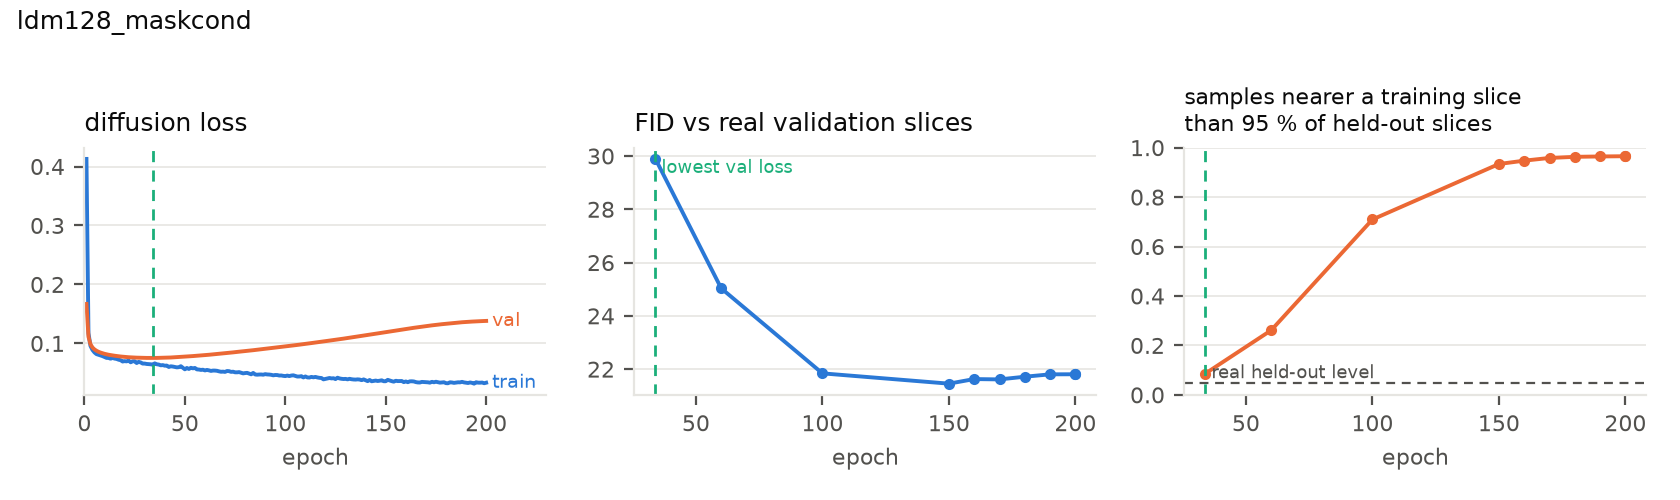
\includegraphics[width=0.92\textwidth]{ldm128_maskcond_checkpoint_curve.png}\\[3pt]
  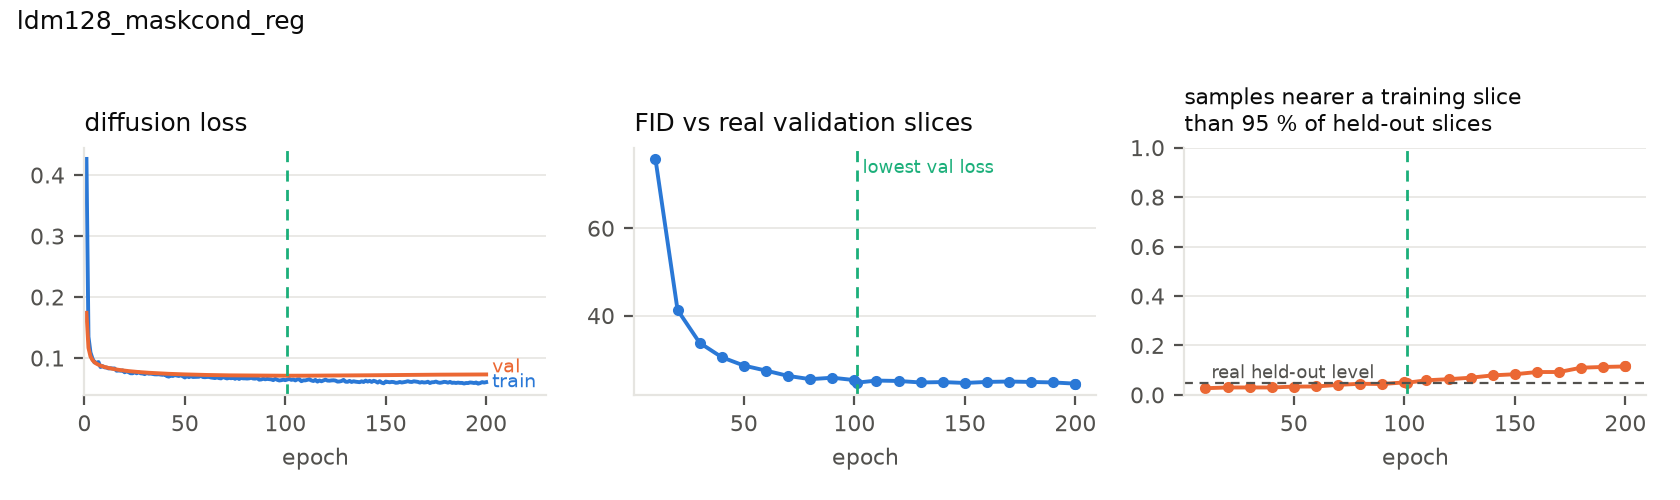
\includegraphics[width=0.92\textwidth]{ldm128_maskcond_reg_checkpoint_curve.png}
  \caption{Validation diffusion loss, FID against real validation slices and memorised fraction per saved checkpoint for the unregularised 128\,px mask-conditioned model (top) and the regularised recipe (bottom). FID keeps improving after the validation-loss minimum in both, but the unregularised model does so by copying: 97\,\% of samples are closer to a training slice than real held-out slices are by epoch~200.}
  \label{fig:curves}
\end{figure}

\begin{table}[t]
  \centering\small
  \caption{Checkpoint curves (2,000 samples per checkpoint, FID vs real validation slices). ``Best'' is the epoch with the lowest validation diffusion loss, the checkpoint used everywhere else. The selection rule (validation data only) picked the reg recipe.}
  \label{tab:curves}
  \resizebox{\textwidth}{!}{\begin{tabular}{lrrrrrr}
    \toprule
    model & best epoch & FID$_\text{val}$ & KID$\times10^3$ & memorised & FID$_\text{val}$ @200 & memorised @200 \\
    \midrule
    \ldm{128}-mask (flips only) & 34 & 29.89 & 18.18 & 0.086 & 21.81 & \textbf{0.966} \\
    \ \ + dropout 0.1 & 41 & 28.82 & 17.24 & 0.093 & 21.99 & \textbf{0.891} \\
    \ \ + dropout 0.1 + affine augmentation (reg, chosen) & 101 & \textbf{24.65} & \textbf{12.86} & \textbf{0.049} & 24.43 & 0.115 \\
    \ldm{128}-reg (unconditional) & 116 & 24.81 & 15.87$^\dagger$ & 0.040 & 23.20 & 0.051 \\
    \ldm{256}-mask-reg & 71 & 15.10 & -- & 0.033 & 12.94 & 0.291 \\
    \bottomrule
  \end{tabular}}\\[2pt]
  {\footnotesize $^\dagger$KID of the unconditional model is against the test slices (Table~\ref{tab:gen}); the curve records FID only.}
\end{table}

Figure~\ref{fig:curves} and Table~\ref{tab:curves} characterise how long training remains credible under the memorisation check. The baseline reaches its lowest validation loss at epoch~34; by epoch~200 its FID against real validation slices has fallen from 29.9 to 21.8, an improvement an FID-only selection rule would take, while 97\,\% of its samples then lie closer to a training slice than 95\,\% of real held-out slices do. Dropout alone changes little (0.891 memorised at epoch~200). Cached affine augmentation postpones the turn to epoch~101, lowers the memorised fraction at the last epoch to 0.115 and gives the best early-stopped model (FID 24.7 vs 28.8 and 29.9). Even so, the regularised 256\,px model starts copying after epoch $\approx 90$ (0.074 at epoch~100, 0.291 at epoch~200): augmentation postpones memorisation, it does not remove it, and early stopping on validation loss remains necessary. All results below use the best-validation-loss checkpoint.

\subsection{Distributional fidelity, diversity, and unseen-mask generation}
\label{sec:gen}
\begin{table}[t]
  \centering\small
  \caption{Generation quality against all 4,623 real test slices (5,000 samples; best-validation-loss EMA weights; DDIM 50). The FID between real validation and real test slices is 10.49 (128\,px) and 9.55 (256\,px); real pair-SSIM is 0.652 / 0.690. Per-modality FIDs replicate one grey channel to RGB and are far above the composite.}
  \label{tab:gen}
  \resizebox{\textwidth}{!}{\begin{tabular}{llrrcrr}
    \toprule
    model & setting & FID & KID$\times10^3$ & FID FLAIR / T1ce / T2 & pair-SSIM & memorised \\
    \midrule
    \ldm{128}-mask (baseline) & $g{=}2$ & 26.22 & 20.89 & 45.9 / 45.4 / 73.0 & 0.576 & 0.069 \\
    \ldm{128}-mask + dropout & $g{=}2$ & 24.34 & 19.13 & 47.7 / 46.2 / 75.7 & 0.585 & 0.070 \\
    \ldm{128}-mask-reg & $g{=}2$ & 20.85 & 15.19 & 44.3 / 44.0 / 69.6 & 0.584 & 0.043 \\
    \ldm{128}-mask-reg & $g{=}1$ & 20.37 & 14.74 & 47.0 / 44.2 / 69.4 & 0.586 & 0.036 \\
    \ldm{128}-mask-reg & $g{=}2$, unseen masks & 22.85 & 16.52 & 45.2 / 44.1 / 71.1 & 0.593 & 0.040 \\
    \ldm{128}-reg (unconditional) & $g{=}1$ & 21.31 & 15.87 & 47.5 / 45.0 / 68.7 & 0.579 & 0.027 \\
    \midrule
    \ldm{256}-mask-reg & $g{=}2$ & \textbf{10.45} & \textbf{6.40} & 40.3 / 39.6 / 59.1 & 0.628 & 0.030 \\
    \ldm{256}-mask-reg & $g{=}1$ & 12.83 & 8.77 & 43.1 / 41.7 / 58.2 & 0.637 & 0.021 \\
    \ldm{256}-mask-reg & $g{=}2$, unseen masks & 10.83 & 6.17 & 40.4 / 39.3 / 60.7 & 0.633 & 0.024 \\
    \bottomrule
  \end{tabular}}
\end{table}

\begin{figure}[t]
  \centering
  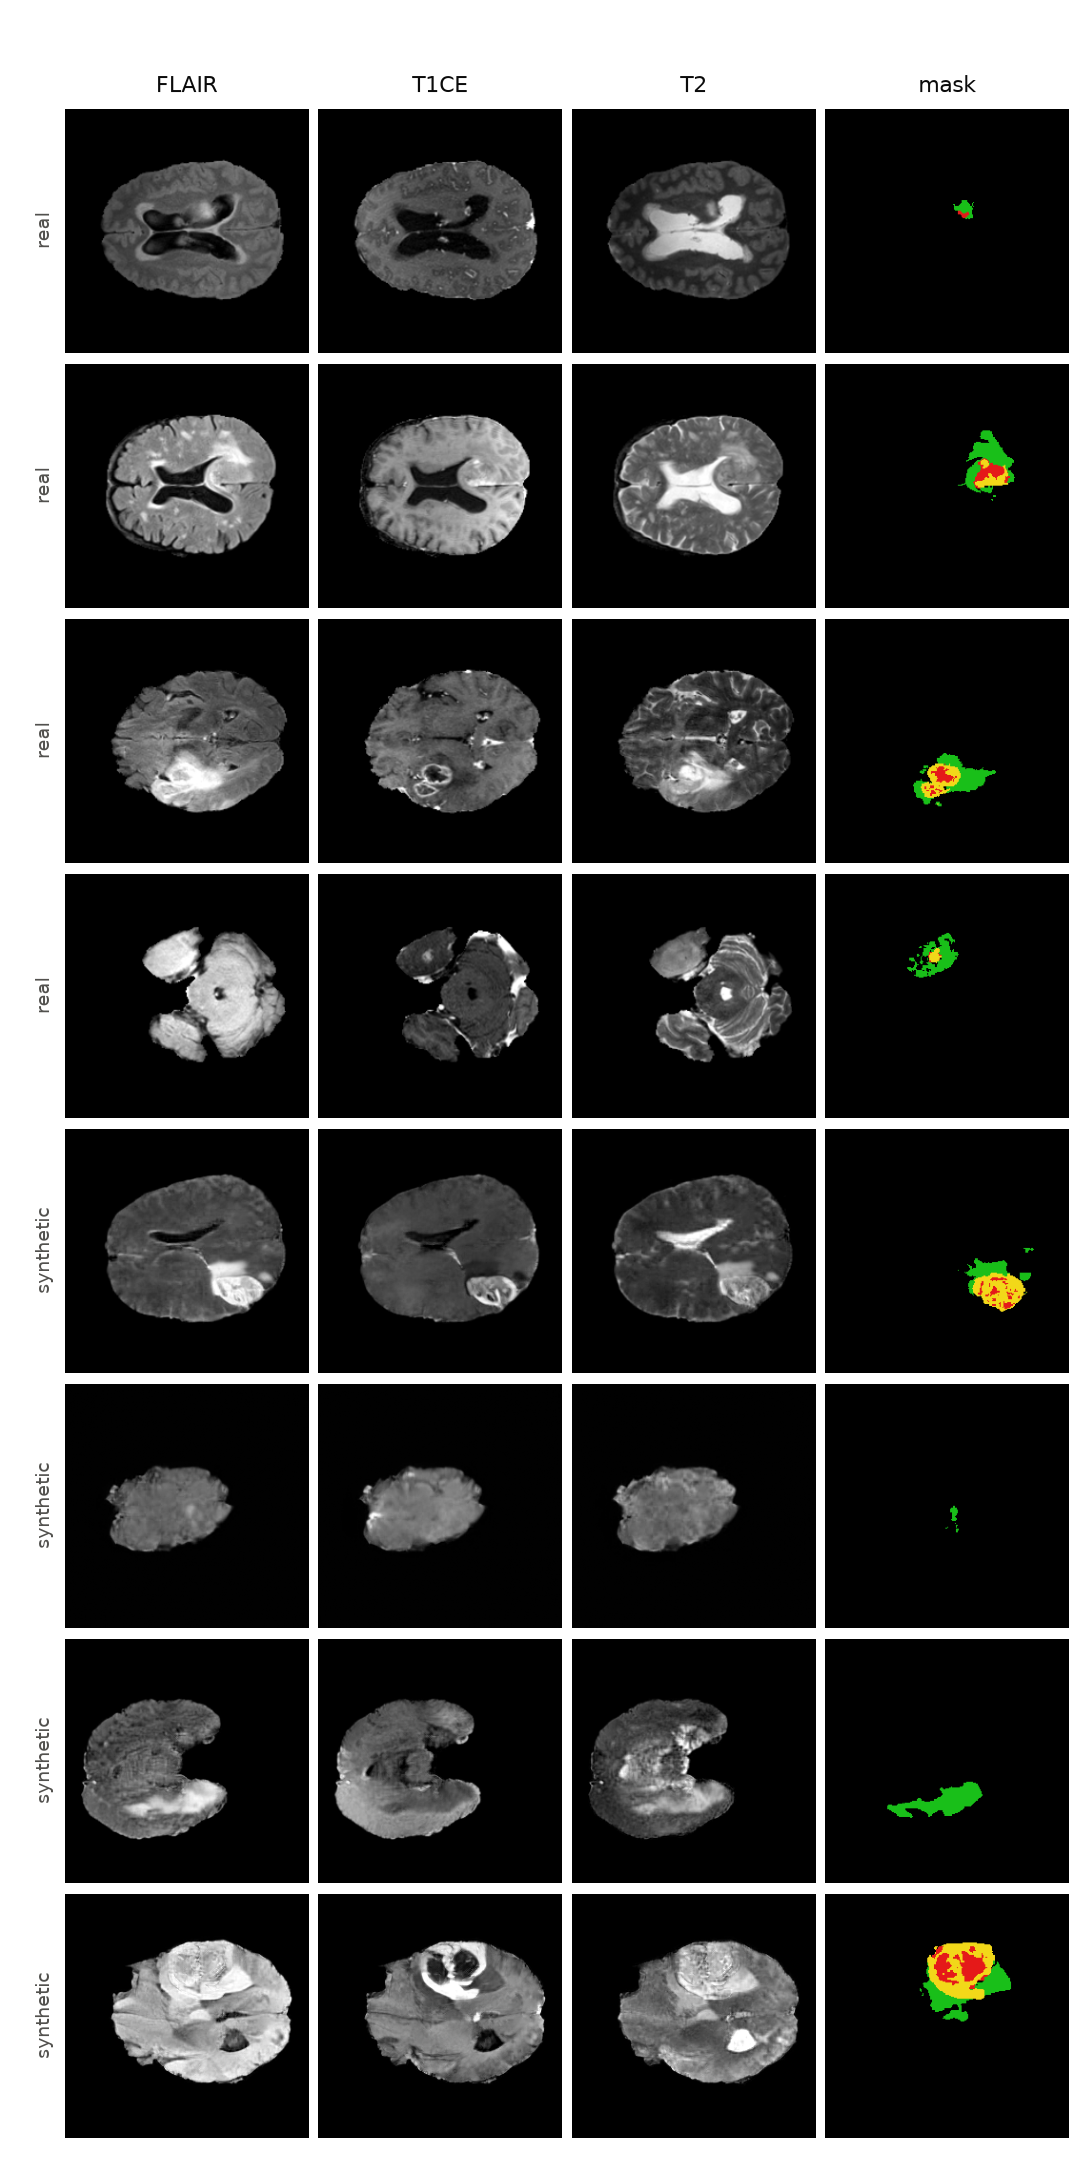
\includegraphics[height=0.42\textheight]{ldm256_maskcond_reg_samples_best_ddim50_cfg2_seed0_real_vs_synth.png}
  \caption{Real test slices (top four rows) and \ldm{256}-mask-reg samples (bottom four rows) with their masks. Colours: necrotic core, oedema, enhancing tumour.}
  \label{fig:samples}
\end{figure}

Table~\ref{tab:gen} scores the early-stopped models on the held-out patients. The regularised recipe improves test FID by 5.4 points over the baseline at 128\,px. Masks of validation patients, tumour shapes never seen in training, cost 2.0 FID points at 128\,px and 0.4 at 256\,px; together with the nearest-neighbour results, this is consistent with conditional generation beyond the training masks, although it is not an anatomical validation. Conditioning costs no fidelity (the mask-conditioned and unconditional 128\,px models score alike), guidance 2 helps at 256\,px and is marginally worse than guidance 1 at 128\,px, and every selected checkpoint has a memorised fraction at or below the 0.05 expected of a model that generalises under this statistic. At 256\,px the model reaches FID 10.45 against a floor of 9.55 between two sets of \emph{real} slices (Fig.~\ref{fig:samples}), encouraging distributional evidence within this dataset rather than proof of clinical realism. T2 is the hardest modality at both resolutions. The autoencoder ceiling is PSNR 26.4\,dB / SSIM 0.833 / LPIPS 0.041 at 128\,px and 29.0\,dB / 0.877 / 0.036 at 256\,px; every latent model remains bounded by this reconstruction stage.

\subsection{Secondary assessment: segmentation utility at 128\,px}
\label{sec:seg}
\begin{table}[t]
  \centering\small
  \caption{Per-patient test Dice at 128\,px (74 test patients; mean $\pm$ std over 3 seeds). Synthetic pairs come from \ldm{128}-mask-reg and are patient-matched.}
  \label{tab:seg128}
  \resizebox{\textwidth}{!}{\begin{tabular}{lrrrcccc}
    \toprule
    training data & patients & real slices & synthetic & WT & TC & ET & mean \\
    \midrule
    10\,\% real & 26 & 1,483--1,705 & 0 & 0.801 $\pm$ 0.011 & 0.580 $\pm$ 0.023 & 0.509 $\pm$ 0.022 & 0.630 $\pm$ 0.016 \\
    10\,\% real + synthetic & 26 & 1,483--1,705 & 1,845--2,208 & 0.809 $\pm$ 0.006 & 0.559 $\pm$ 0.010 & 0.430 $\pm$ 0.033 & 0.600 $\pm$ 0.014 \\
    25\,\% real & 64 & 3,937--4,031 & 0 & 0.847 $\pm$ 0.003 & 0.676 $\pm$ 0.011 & 0.611 $\pm$ 0.010 & 0.711 $\pm$ 0.004 \\
    25\,\% real + synthetic & 64 & 3,937--4,031 & 4,913--5,158 & 0.844 $\pm$ 0.004 & 0.660 $\pm$ 0.021 & 0.521 $\pm$ 0.014 & 0.675 $\pm$ 0.012 \\
    100\,\% real & 258 & 15,895 & 0 & 0.886 $\pm$ 0.001 & 0.775 $\pm$ 0.005 & 0.673 $\pm$ 0.004 & 0.778 $\pm$ 0.003 \\
    100\,\% real + synthetic & 258 & 15,895 & 20,000 & 0.879 $\pm$ 0.001 & 0.742 $\pm$ 0.009 & 0.650 $\pm$ 0.010 & 0.757 $\pm$ 0.006 \\
    synthetic only & 0 & 0 & 20,000 & 0.829 $\pm$ 0.002 & 0.669 $\pm$ 0.007 & 0.481 $\pm$ 0.012 & 0.660 $\pm$ 0.005 \\
    \bottomrule
  \end{tabular}}
\end{table}

\begin{figure}[t]
  \centering
  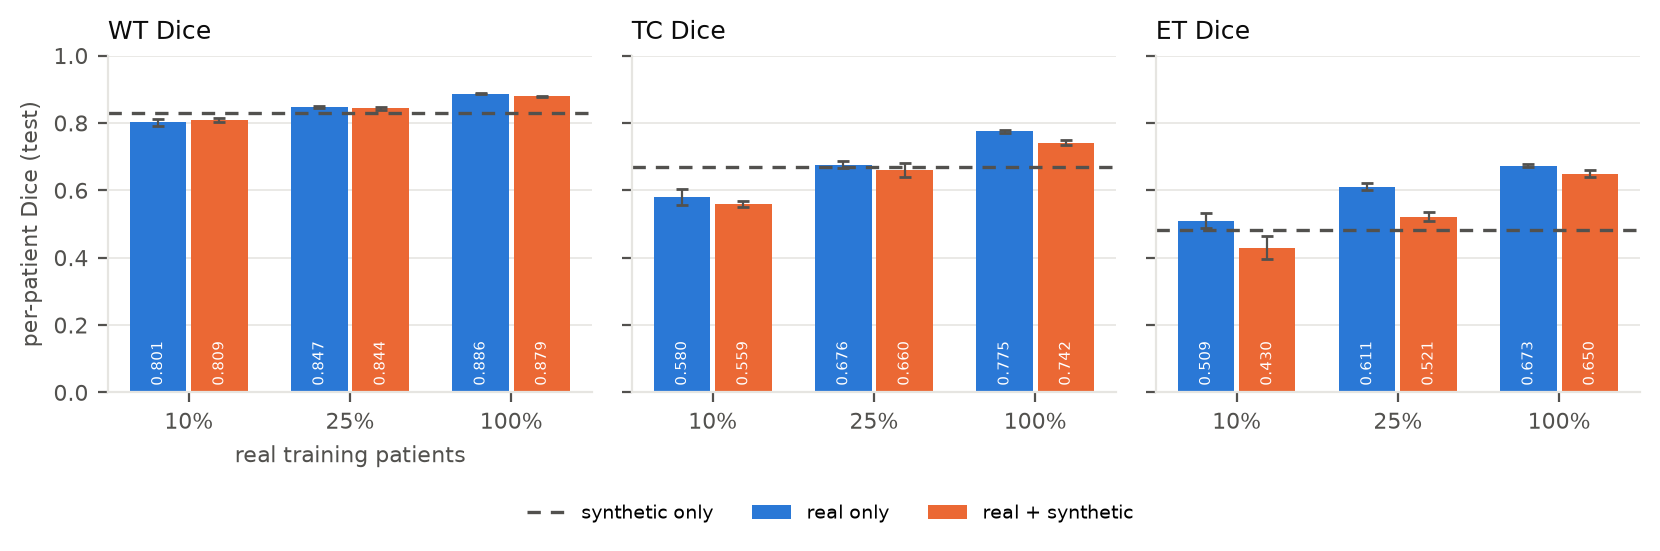
\includegraphics[width=\textwidth]{segmentation_dice.png}
  \caption{128\,px primary protocol: per-patient test Dice with and without patient-matched synthetic pairs, three seeds. The dashed line is the synthetic-only segmenter.}
  \label{fig:seg128}
\end{figure}

Mixing the synthetic pairs into training did not improve the segmenter (Table~\ref{tab:seg128}, Fig.~\ref{fig:seg128}). Whole-tumour Dice rises slightly with 26 real patients (0.801 $\to$ 0.809), but TC and ET fall at every fraction (ET at 10\,\%: 0.509 $\to$ 0.430; mean Dice at 100\,\%: 0.778 $\to$ 0.757), and the loss is present in 9 of 9 seed-matched pairs. Synthetic data alone reaches 0.660 mean Dice, about the level of 26 real patients. Mask consistency helps localise where the loss sits: a real-trained segmenter recovers the whole-tumour outline of the synthetic images well (WT consistency 0.789 for the 100\,\% segmenter, vs 0.886 on real test slices) but agrees with the conditioning mask on ET only about half the time (0.494). The pairs retain the tumour outline but appear to weaken the TC/ET signal that the segmenter uses.

\subsection{Secondary analyses of segmentation utility}
\label{sec:secondary}
\begin{table}[t]
  \centering\small
  \caption{Secondary analyses at 128\,px: change in mean test Dice relative to real only, seed-matched, three seeds (per-region changes for the two decisive rows). The control row pre-trains for the same 20 extra epochs on the real slices.}
  \label{tab:secondary}
  \resizebox{\textwidth}{!}{\begin{tabular}{lccc}
    \toprule
    condition & 10\,\% real & 25\,\% real & 100\,\% real \\
    \midrule
    real + synthetic, 1.25:1 (primary) & $-0.030$ & $-0.036$ & $-0.021$ \\
    real + synthetic, 1:1 & $-0.020$ & $-0.024$ & $-0.018$ \\
    real replaced by its frozen-VAE reconstruction (no generator) & $-0.057$ (ET $-0.112$) & $-0.072$ (ET $-0.135$) & $-0.072$ (ET $-0.131$) \\
    synthetic pre-training, then real & $\mathbf{+0.044}$ & $\mathbf{+0.015}$ & $+0.001$ \\
    real pre-training, then real (compute-matched control) & $+0.023$ & $+0.001$ & $+0.004$ \\
    synthetic pre-training $-$ control & $\mathbf{+0.021}$ (3/3 seeds) & $\mathbf{+0.014}$ (3/3 seeds) & $-0.003$ \\
    \bottomrule
  \end{tabular}}
\end{table}

\begin{figure}[t]
  \centering
  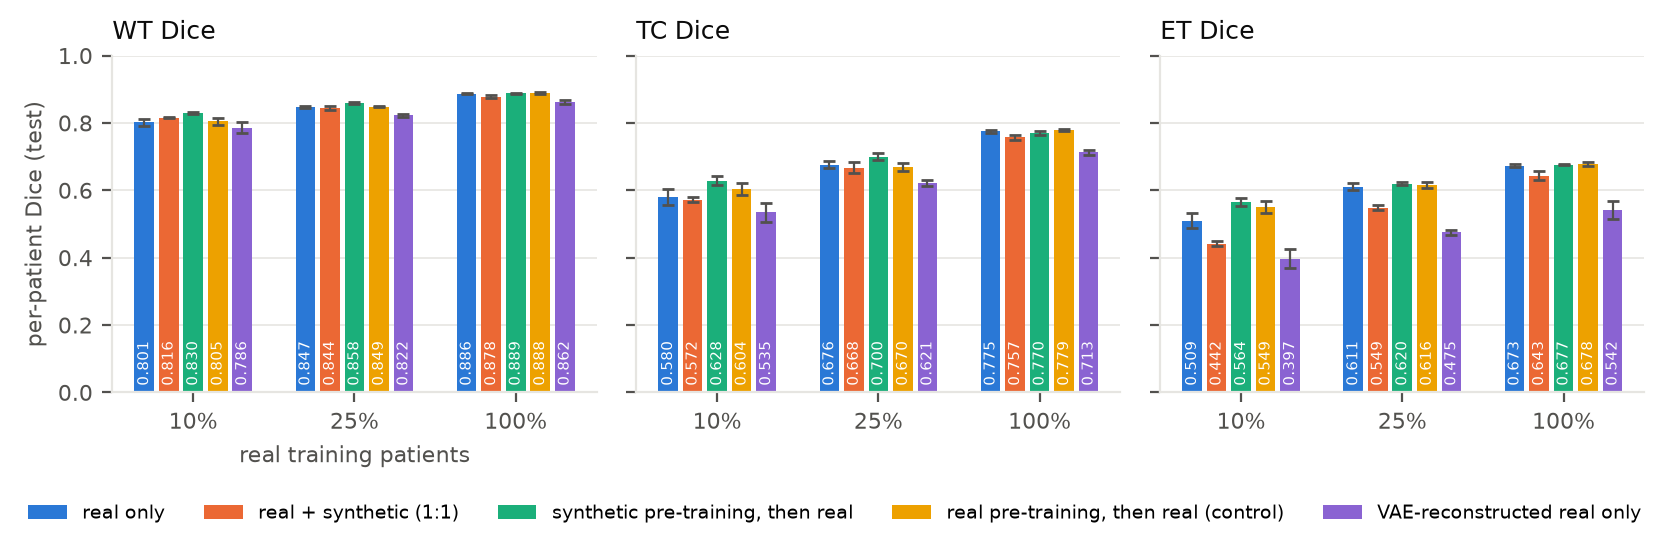
\includegraphics[width=\textwidth]{segmentation_dice_secondary.png}
  \caption{128\,px secondary analyses (frozen decoder): real only, real + synthetic 1:1, synthetic pre-training, real pre-training (control) and real slices reconstructed through the frozen autoencoder.}
  \label{fig:secondary}
\end{figure}

Table~\ref{tab:secondary} and Fig.~\ref{fig:secondary} explore the three questions declared after the first seed-0 results. \emph{Changing the ratio is insufficient}: capping synthetic slices at 1:1 recovers only about a third of the loss and ET stays 0.03--0.07 below real-only. \emph{The frozen autoencoder reproduces the loss without a generator}: replacing the real slices by their own reconstruction through \texttt{sd-vae-ft-mse} costs $-0.057$ / $-0.072$ / $-0.072$ mean Dice, again concentrated on ET ($-0.11$ to $-0.14$). Because every synthetic image passes through this autoencoder, the result is consistent with important enhancing-tumour information being lost before diffusion sampling. \emph{Pre-training helps where mixing does not}: 20 epochs on synthetic pairs followed by the standard schedule on real data gains $+0.044$ mean Dice with 26 patients (all three regions, ET 0.509 $\to$ 0.564, 3/3 seeds) and $+0.015$ with 64, nothing with 258. Because the pre-trained segmenter sees 20 extra epochs, a control was declared that spends those epochs on the real slices: it recovers about half of the 10\,\% gain and none of the 25\,\% gain, leaving a synthetic-specific effect of $+0.021$ and $+0.014$ (3/3 seeds each). This pattern suggests that real-data fine-tuning can override synthetic-image limitations while retaining some transferable signal.

\subsection{Resolution as a boundary condition: segmentation at 256\,px}
\label{sec:256}
\begin{table}[t]
  \centering\small
  \caption{Per-patient test Dice at 256\,px with the \ldm{256}-mask-reg pool (same protocol, seeds and patient matching as Table~\ref{tab:seg128}).}
  \label{tab:seg256}
  \begin{tabular}{lccccr}
    \toprule
    training data & WT & TC & ET & mean & $\Delta$ mean \\
    \midrule
    10\,\% real & 0.849 $\pm$ 0.006 & 0.672 $\pm$ 0.019 & 0.604 $\pm$ 0.009 & 0.709 $\pm$ 0.003 & \\
    10\,\% real + synthetic & 0.860 $\pm$ 0.006 & 0.721 $\pm$ 0.007 & 0.626 $\pm$ 0.006 & 0.736 $\pm$ 0.004 & $\mathbf{+0.027}$ \\
    25\,\% real & 0.874 $\pm$ 0.003 & 0.751 $\pm$ 0.009 & 0.668 $\pm$ 0.010 & 0.764 $\pm$ 0.007 & \\
    25\,\% real + synthetic & 0.878 $\pm$ 0.000 & 0.769 $\pm$ 0.004 & 0.654 $\pm$ 0.000 & 0.767 $\pm$ 0.001 & $+0.003$ \\
    100\,\% real & 0.895 $\pm$ 0.000 & 0.810 $\pm$ 0.002 & 0.707 $\pm$ 0.002 & 0.804 $\pm$ 0.000 & \\
    100\,\% real + synthetic & 0.894 $\pm$ 0.004 & 0.818 $\pm$ 0.006 & 0.692 $\pm$ 0.008 & 0.801 $\pm$ 0.005 & $-0.003$ \\
    synthetic only & 0.871 $\pm$ 0.002 & 0.785 $\pm$ 0.008 & 0.623 $\pm$ 0.004 & 0.760 $\pm$ 0.003 & \\
    \bottomrule
  \end{tabular}
\end{table}

The primary protocol was repeated unchanged at 256\,px, declared before any 256\,px segmenter was trained (Table~\ref{tab:seg256}). With 26 real patients the sign flips: the patient-matched synthetic pairs improve every region (TC $+0.049$, ET $+0.022$, WT $+0.011$; 3/3 seeds, spread $\le 0.004$), where the same protocol at 128\,px lost 0.030. With 64 patients the effect is neutral and with 258 it is neutral on the mean and still slightly negative on ET ($-0.015$). The synthetic-only segmenter reaches 0.760, the level of 25\,\% real data (128\,px: 0.660, the level of 10\,\%). The 256\,px pool comes from a generator at the FID floor decoded through an autoencoder whose ceiling is 2.6\,dB higher; the real-only segmenters are stronger at 256\,px as well, so the two resolutions are compared only within themselves.

\subsection{Autoencoder as a boundary condition: decoder fine-tuning}
\label{sec:decoder}
\begin{figure}[t]
  \centering
  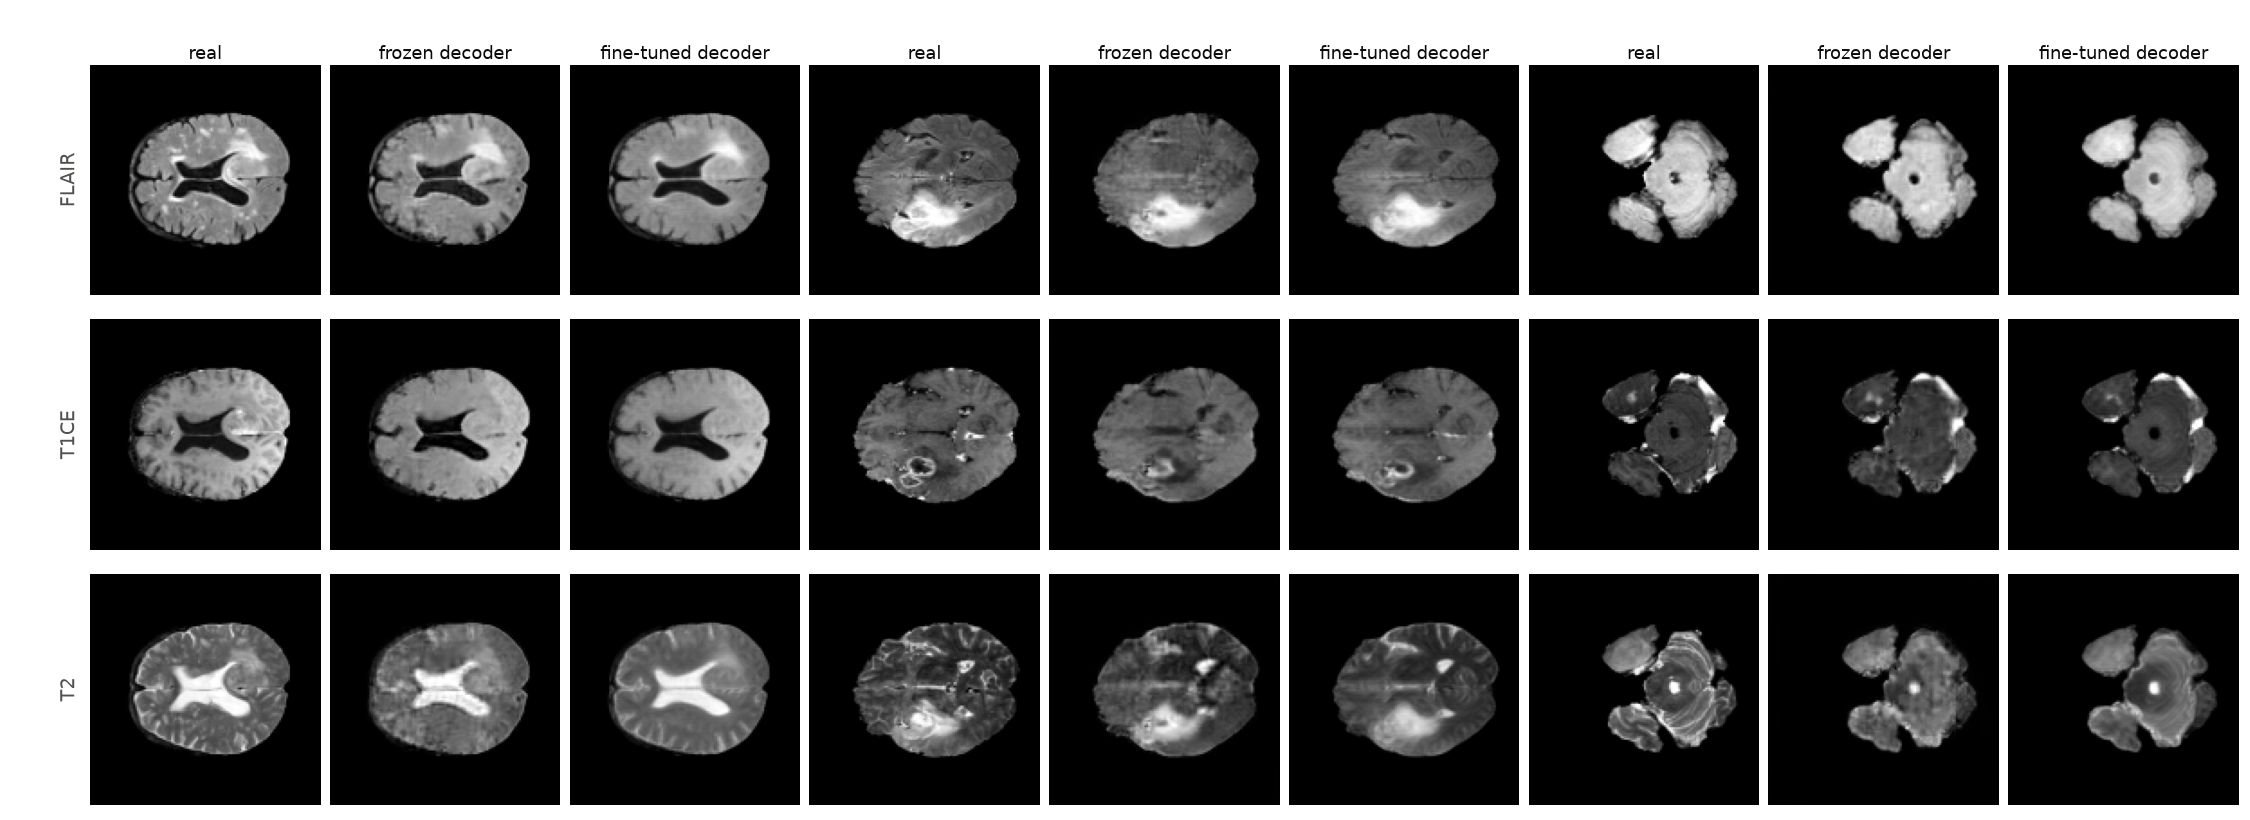
\includegraphics[width=\textwidth]{vae_decoder_brats128.png}
  \caption{Three test slices with enhancing tumour reconstructed through the frozen and the fine-tuned decoder (same encoder, same latents). The blotchy texture the frozen decoder adds to T2 disappears and enhancing rims in T1ce come out sharper.}
  \label{fig:decoder}
\end{figure}

\begin{table}[t]
  \centering\small
  \caption{Decoder fine-tuning at 128\,px. Top: reconstruction ceiling on the 4,623 test slices and scores of the \emph{same} 20,000 latent samples decoded with each decoder. Bottom: change in mean test Dice relative to real only (seed-matched, three seeds) when the segmentation protocols are repeated with the re-decoded pool.}
  \label{tab:decoder}
  \resizebox{\textwidth}{!}{\begin{tabular}{lcccccc}
    \toprule
    & PSNR & SSIM & LPIPS & FID (3-ch) & FID FLAIR / T1ce / T2 & memorised \\
    \midrule
    frozen decoder & 26.37\,dB & 0.833 & 0.041 & 20.85 & 44.3 / 44.0 / 69.6 & 0.043 \\
    fine-tuned decoder & \textbf{27.79\,dB} & \textbf{0.883} & \textbf{0.032} & 20.89 & \textbf{28.6 / 25.6 / 17.6} & 0.051 \\
    \midrule
    $\Delta$ mean Dice vs real only & \multicolumn{2}{c}{10\,\% real} & \multicolumn{2}{c}{25\,\% real} & \multicolumn{2}{c}{100\,\% real} \\
    \cmidrule(lr){2-3}\cmidrule(lr){4-5}\cmidrule(lr){6-7}
    & frozen & fine-tuned & frozen & fine-tuned & frozen & fine-tuned \\
    \midrule
    real + synthetic (1.25:1) & $-0.031$ & $-0.020$ & $-0.036$ & $-0.033$ & $-0.021$ & $-0.012$ \\
    \ \ ET only & $-0.079$ & $-0.064$ & $-0.089$ & $-0.081$ & $-0.024$ & $-0.022$ \\
    real + synthetic (1:1) & $-0.020$ & $-0.007$ & $-0.024$ & $-0.025$ & $-0.018$ & $-0.012$ \\
    real replaced by its VAE reconstruction & $-0.057$ & $-0.044$ & $-0.072$ & $-0.055$ & $-0.072$ & $-0.045$ \\
    \ \ ET only & $-0.112$ & $-0.080$ & $-0.135$ & $-0.107$ & $-0.131$ & $-0.089$ \\
    synthetic pre-training $-$ control & $+0.021$ & $+0.018$ & $+0.014$ & $+0.015$ & $-0.003$ & $-0.001$ \\
    synthetic only (mean Dice) & \multicolumn{2}{c}{0.660 $\to$ 0.672} & & & & \\
    \bottomrule
  \end{tabular}}
\end{table}

Fine-tuning the decoder on the training slices improves every image metric (Table~\ref{tab:decoder}, Fig.~\ref{fig:decoder}): the ceiling rises from 26.37 to 27.79\,dB (SSIM 0.833 $\to$ 0.883, LPIPS 0.041 $\to$ 0.032; T2, the worst channel, gains 1.6\,dB), so reading (a) passed and the study continued. Decoding the same 20,000 latents again leaves the three-channel FID unchanged (20.85 $\to$ 20.89) but cuts the per-modality FIDs by 35--75\,\% (T2 69.6 $\to$ 17.6); the per-channel scores of the frozen decoder were dominated by the texture it invents, which the composite metric, seeing the three channels as one colour image, largely ignores. Sample diversity moves towards that of real slices (pair-SSIM 0.584 $\to$ 0.636, real 0.652), and the memorised fraction rises from 0.043 to 0.051 because every sample moves closer to every real slice under a sharper decoding; the latents are identical, so this is not new copying.

The segmenter, however, barely notices. With the re-decoded pool, mixing still costs Dice at every fraction and in 9 of 9 seed-matched pairs ($-0.020$ / $-0.033$ / $-0.012$; ET still $-0.06$ to $-0.08$), the re-trained real-only baselines reproduce the earlier ones within the seed spread, and the synthetic-only segmenter improves from 0.660 to 0.672. The VAE-reconstructed-real control moves towards real-only at every fraction ($-0.057$ / $-0.072$ / $-0.072$ $\to$ $-0.044$ / $-0.055$ / $-0.045$) and real + synthetic moves the same way, so the pre-declared condition (b) is met, but only in part: a decoder trained on these very slices still loses 0.044--0.055 mean Dice (ET 0.08--0.11) when real slices are merely passed through the autoencoder, which remains more than mixing costs. Within this setup, the controls are consistent with the autoencoder being the principal limitation and with most of that limitation arising in the encoder's $16\times16\times4$ latent rather than the decoder; the decoder accounts for about a third of the observed loss. The pre-training gain is unchanged by the decoder ($+0.018$ / $+0.015$ against the control).

\FloatBarrier
\section{Discussion}
\paragraph{Viability assessment.} The results support a limited and conditional account of viability rather than a general claim that latent diffusion solves synthetic brain MRI generation. Training and sampling are technically feasible in the tested 2-D setting, and the 256\,px model provides encouraging distributional evidence relative to held-out data. That evidence depends on regularisation and validation-based early stopping: prolonged training improves FID while increasingly reproducing the training set. Generation from unseen-patient masks adds preliminary same-dataset evidence of conditional generalisation, while the segmentation experiments show that practical utility depends on resolution and on how the synthetic pairs are used.

\begin{table}[t]
  \centering\small
  \setlength{\tabcolsep}{4pt}
  \renewcommand{\arraystretch}{1.08}
  \caption{What the exploratory study does and does not establish. ``Supported'' is restricted to the reported 2-D BraTS~2020 setting.}
  \label{tab:viability}
  \begin{tabular}{@{}>{\raggedright\arraybackslash}p{0.17\textwidth}>{\raggedright\arraybackslash}p{0.22\textwidth}>{\raggedright\arraybackslash}p{0.23\textwidth}>{\raggedright\arraybackslash}p{0.28\textwidth}@{}}
    \toprule
    dimension & evidence & finding & interpretation \\
    \midrule
    Technical feasibility & Training and sampling at 128 and 256\,px & Both resolutions produced reproducible model outputs & Supported for the tested pipeline \\
    Distributional fidelity & FID/KID and a real-vs-real reference & 256\,px FID 10.45 vs a 9.55 reference & Encouraging metric-based evidence \\
    Diversity and non-copying & Pair-SSIM and nearest-neighbour fraction & Selected checkpoints remain near the held-out reference; late checkpoints copy & Conditional on augmentation and early stopping \\
    Unseen-mask generation & 5,000 samples from validation-patient masks & Small FID change relative to training-patient masks & Preliminary support within the same dataset \\
    Segmentation utility & Patient-matched, three-seed experiments & 128\,px mixing hurts; low-data pre-training and 256\,px mixing can help & Conditional rather than general utility \\
    Clinical validity & No radiologist study or external cohort & Not measured & Not established \\
    \bottomrule
  \end{tabular}
\end{table}
\FloatBarrier

\paragraph{What the results suggest.} A latent diffusion model built on a natural-image autoencoder can produce BraTS slices with strong held-out fidelity scores while still developing a serious memorisation risk during prolonged training. At 128\,px, the no-generator and decoder controls are consistent with the autoencoder bottleneck weakening the enhancing-tumour information needed for segmentation; improved image metrics after decoder fine-tuning do not remove the downstream loss. Two settings provide evidence of conditional utility: synthetic pre-training followed by real-data fine-tuning, and mixing at 256\,px in the low-data regime. These are boundary observations, not evidence that synthetic augmentation will help across datasets, architectures or clinical tasks.

\paragraph{Implications for evaluation.} Three practices were decisive and are cheap: early stopping on the validation diffusion loss with a memorisation check, since FID alone would have chosen the most memorised checkpoints; a no-generator control (real slices through the autoencoder), which localised the loss; and a compute-matched control for pre-training, which halved the apparent gain. Per-modality FIDs and the composite FID also disagree sharply once the decoder changes, so a single FID number is not a safe summary for multi-channel medical images.

\paragraph{Limitations and what remains untested.} All models are 2-D and Dice is aggregated per patient over slices, not on volumes. FID/KID use Inception features; the real val-vs-test floor calibrates them, but a radiology-specific extractor~\citep{mei2022radimagenet} would be more sensitive to clinically relevant detail. No radiologist evaluated anatomical or diagnostic plausibility, and there is no privacy analysis or external test cohort. The encoder of the autoencoder is frozen; a medical-image autoencoder or an encoder fine-tune with the diffusion models retrained is the natural next experiment, and the present controls suggest it may matter more than decoder-only fine-tuning. The segmenter is a plain 2-D U-Net rather than a tuned nnU-Net~\citep{isensee2021nnunet}, and the evidence comes from one dataset, one patient split and three segmentation seeds. The study therefore motivates further 3-D, external-dataset and expert-reader evaluation rather than clinical use.

\FloatBarrier
\section{Conclusion}
Within the tested 2-D BraTS~2020 setting, latent diffusion is a plausible research pipeline for synthetic brain MRI generation, but its viability is conditional. Cached affine augmentation and validation-based early stopping are needed to control memorisation; higher resolution produces substantially stronger distributional evidence; and downstream value depends on whether the samples are mixed directly or used for pre-training before real-data fine-tuning. The controls suggest that the pretrained autoencoder, particularly its compressed latent representation at 128\,px, is an important boundary on useful detail. These results justify further study of medical-image autoencoders, 3-D generation, external datasets and expert assessment, but they do not establish broad segmentation benefit or clinical validity. We release the code, patient split, pre-declared protocol and every run's configuration and metrics so that this exploratory assessment can be reproduced and extended.

\paragraph{Reproducibility.} Code, split file, protocol declarations with timestamps, result tables and figures: \url{https://github.com/wasiqnauman/SynthMRI}. One command reproduces the full experiment set on a single 16\,GB GPU in about 40 hours; every reported number is traceable to a run directory that records the resolved configuration, git commit and metrics.

\bibliographystyle{plainnat}
\bibliography{refs}
\end{document}
